\Transcb{yellow}{blue}{Samenvatting en Vooruitzichten}
\onecolumn
\begin{itemize}
\item {\blue IceCube : 's Werelds grootste neutrino observatorium op de Zuidpool}
\item[] De volledige IceCube detector is sinds december 2010 in bedrijf
\item[] IceCube sensoren werken naar behoren (Maanschaduw, hemelkaart)
\item \colorbox{yellow}{Wereldprimeur (2013): Kosmische hoog-energetische neutrino's ontdekt}
\item[] \begin{center}{\red De geboorte van Neutrino Astronomie}\end{center}
\item {\blue Ligo-Virgo : 's Werelds eerste observatorium voor gravitatiegolven}
\item[] \colorbox{yellow}{Wereldprimeur (2015): Ontdekking van gravitatiegolven}
\item[] Waargenomen signalen van samensmeltende zwarte gaten en neutronensterren
\item \colorbox{yellow}{Wereldprimeur (2018): Eerste kosmische neutrinobron ge\"{i}dentificeerd}
\item[] Neutrino alarm (IceCube) $\rightarrow$ Opflakkerende Blazar (Fermi, Magic)
\item[] {\blue Gecombineerd onderzoek van het "Gamma, Neutrino, GW Universum"}
\item \colorbox{yellow}{Uitbreiding naar hogere neutrino energie (radio detectie)}
\end{itemize}
%
\begin{center}
{\red \shabox{Er breken zeer interessante tijden aan voor onze Astrodeeltjes Fysica !}}
\end{center}

\Tr
\onecolumn
\begin{center}
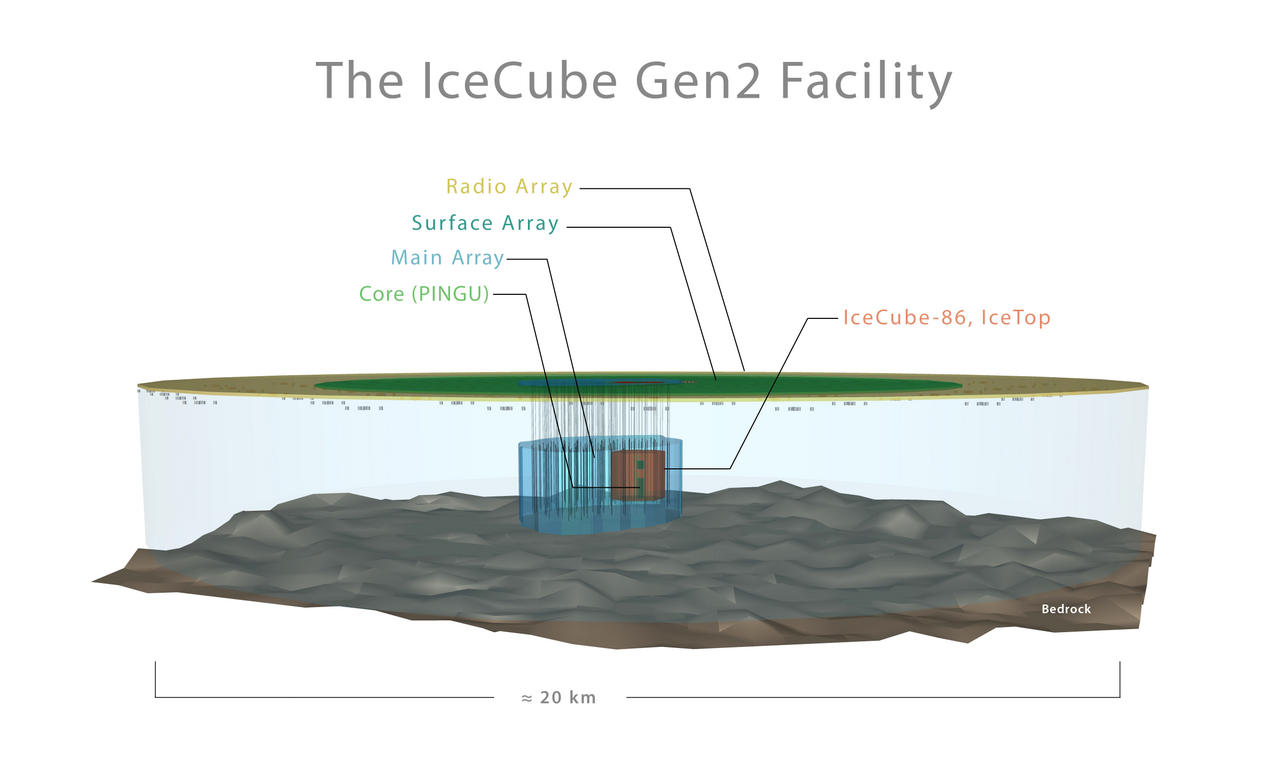
\includegraphics[keepaspectratio,height=15cm]{icecube-gen2}
\end{center}
